\PassOptionsToPackage{american}{babel}
\documentclass[twoside]{article}
\usepackage[american]{babel}
\usepackage[backend=biber,style=apa,sortcites=true,sorting=nyt]{biblatex}
\DeclareLanguageMapping{american}{american-apa}
\addbibresource{./Transenvironmental.bib}
\usepackage{capt-of}
\usepackage{longtable}
\usepackage{setspace}
\usepackage{etoolbox}
\AtBeginEnvironment{longtable}{\singlespacing}
\usepackage{fancyhdr}
\fancyhead[LE,RO]{Mainstream Decision Tree}
\fancyhead[LO,RE]{Michael Ryan Hunsaker, PhD}
\pagestyle{fancy}
\usepackage{booktabs}
\usepackage{float}
\usepackage{afterpage}
\usepackage{caption}
\usepackage{blindtext}
\usepackage{tabularx}
\usepackage{graphicx}
\graphicspath{ {images/} }
\usepackage[toc,page]{appendix}
\usepackage{pdfpages}
\usepackage{csquotes}
\usepackage{setspace}
\usepackage{geometry}
\usepackage{bookman} 
\usepackage{endnotes}
\usepackage{url}
\usepackage{lscape}
\usepackage{authblk}
\usepackage{listings}
\usepackage{listings}
\usepackage{color}
\lstset{ %
	language=R,                     % the language of the code
	basicstyle=\footnotesize,       % the size of the fonts that are used for the code
	numbers=left,                   % where to put the line-numbers
	numberstyle=\tiny\color{gray},  % the style that is used for the line-numbers
	stepnumber=1,                   % the step between two line-numbers. If it's 1, each line
	% will be numbered
	numbersep=5pt,                  % how far the line-numbers are from the code
	backgroundcolor=\color{white},  % choose the background color. You must add \usepackage{color}
	showspaces=false,               % show spaces adding particular underscores
	showstringspaces=false,         % underline spaces within strings
	showtabs=false,                 % show tabs within strings adding particular underscores
	frame=single,                   % adds a frame around the code
	rulecolor=\color{black},        % if not set, the frame-color may be changed on line-breaks within not-black text (e.g. commens (green here))
	tabsize=2,                      % sets default tabsize to 2 spaces
	captionpos=b,                   % sets the caption-position to bottom
	breaklines=true,                % sets automatic line breaking
	breakatwhitespace=false,        % sets if automatic breaks should only happen at whitespace
	title=\lstname,                 % show the filename of files included with \lstinputlisting;
	% also try caption instead of title
	keywordstyle=\color{blue},      % keyword style
	commentstyle=\color{green!55!blue},   % comment style
	stringstyle=\color{red!55!black},      % string literal style
	escapeinside={\%*}{*)},         % if you want to add a comment within your code
	morekeywords={*,...}            % if you want to add more keywords to the set
} 
\pagenumbering{gobble}
\DeclareCaptionLabelFormat{adja-page}{\hrulefill\\#1 #2 \emph{(previous page)}}
\DeclareCaptionFont{tiny}{\tiny}
%
\makeatletter
\AtBeginEnvironment{tabular}{%
  \def\baselinestretch{1}\@currsize}%
\makeatother
%
\title{Development and Implementation of a Mainstreaming Process to Transition Students from Self-Contained Special Education into General Education Placements: Part 2 Computational Validation}
%\shorttitle{Mainstreaming Pipeline}
%
\author[1]{Michael Ryan Hunsaker, Ph.D.}
\affil[1]{University of Utah, Salt Lake City, UT, USA}
%
%\rightheader{Mainstreaming Pipeline}
%\leftheader{Michael Ryan Hunsaker, Ph.D.}
%
\begin{document}
%
\maketitle
%
\begin{abstract}
%
%
%
%
%
%
\end{abstract}
%
\section{Introduction}
%
%
%
\section{Methods}
\subsection{Manual Selection of Mainstreaming LRE}
Using the Mainstream Decision Tree and raw data (raw values rather than categorical values), student allocation was determined for each student manually and annotated in a spreadsheet with the rest of the data from the above step using the \textit{Mainstreaming Decision Tree}. These data were later used to evaluate the efficacy of the numerical analyses. See method for manual selection and mainstreaming pipeline in (\textbf{REF to Part 1}).

\subsection{Data Analysis and Development of a Support Vector Machine to Assist in Special Education Student Mainstreaming Allocation}
\subsection{Data Preprocessing}
Data were collected from all students in academic self-contained classroom settings.  student's most recent special education re-evaluation. The following data were extracted: Adaptive Function, Full Scale IQ (FSIQ), SocioEmotional data, WJ-IIINU data for academics (Basic Reading Skills, Reading Comprehension, Math Reasoning, Math Calculation, Written Language) and Curriculum Based Measures (CBM-Math and ELA/Reading). See Table~\ref{tab1} for items extracted from special education files.
%
%%%%%%%%%%%%%%%%%%%%%%%%%%%%%%%%%%%%%%%%%%%%
%
% Begin Table 1
%
%%%%%%%%%%%%%%%%%%%%%%%%%%%%%%%%%%%%%%%%%%%%
%
\begin{table}[tbp!]
	\centering
	\vspace*{0cm}\caption{Data Considered by a Special Education Student Mainstreaming Allocation}
	\label{tab1}
	\resizebox{\textwidth}{!}
	{\begin{tabular}{ccccc}
			\hline\\[-1.5ex]
			Adaptive & Intelligence & \multicolumn{2}{c}{Academic Achievement} & Emotional \\[0.5ex]
			\cmidrule(lr){3-4}
			& & Woodcock Johnson IIINU/IV & Curriculum Based Measurements & \\
			\hline\\[-1.5ex]
			VABS 2/3 & Stanford Binet V & Reading Skills & District Benchmarks & BASC 2/3\\
			ABAS 2/3 & Weschler Nonverbal (WNV) & Reading Comprehension & Utah Compose & Connor's 3\\
			BASC 2/3 (Adaptive) & WISC III/IV/V & Math Calculation & AIMS Web & Achenbach CBCL\\
			& Woodcock Johnson IIINU/IV & Math Reasoning & DRA 2 & \\
			& KBIT 2 & Broad Writing (includes Spelling) & Spelling City & \\
			& Leiter R & Broad Reading & GoMath Benchmark, Chapter Tests & \\
			& UNIT 2 & Broad Math & Eureka Math &\\
			& DAS & & DIBLES Next &\\
			& Batelle & & Success Maker &\\
			& & & Imagine Learning &\\
			& & & Reflex Math &\\
			& & & Common Formative Assessments (CFA) &\\
			& & & \textbf{Any evidence-based measure approved by IEP team} &\\
			\hline
	\end{tabular}}
\end{table}
%
%%%%%%%%%%%%%%%%%%%%%%%%%%%%%%%%%%%%%%%%%%%%
%
% End Table 1
%
%%%%%%%%%%%%%%%%%%%%%%%%%%%%%%%%%%%%%%%%%%%%
%
These values were converted into categorical variables based on the school district rubric for classification as specific learning disability (SLD). The categorical variables are presented in Table ~\ref(tab2)
%
%%%%%%%%%%%%%%%%%%%%%%%%%%%%%%%%%%%%%%%%%%%%
%
% Begin Table 2
%
%%%%%%%%%%%%%%%%%%%%%%%%%%%%%%%%%%%%%%%%%%%%
%
\begin{table}[tbp!]
	\centering
	\caption{Continuous to Categorical Value Mapping}
	\label{tab2}
	\begin{tabular}{ccc}
		\hline \\
		Measure & Value Definitions & Value Range\\
		\hline \\
		Adaptive & SS 0-59 = 0,SS \textgreater60 = 1 & [0,1]\\
		FSIQ & SS 0-70 = 0, SS 70-100 = 1, SS \textgreater100 = 2 & [0,0.5,1]\\
		SocioEmotional & T 0-70 = 0, T\textgreater70 = 1 & [0,1]\\
		WJ-III NU & SS 0-70 \& RPI 0-18 = 0, SS 70-100 \& RPI 18-34 = 1, SS\textgreater100 = 2 & [0,.33,.67,1]\\
		CBM & \textless30\%ile = 0, textgreater30\%ile = 1 &  [0,1]\\
		\hline
	\end{tabular}
\end{table}
%
%%%%%%%%%%%%%%%%%%%%%%%%%%%%%%%%%%%%%%%%%%%%
%
% End Table 2
%
%%%%%%%%%%%%%%%%%%%%%%%%%%%%%%%%%%%%%%%%%%%%
%
\subsubsection{Regression Tree Analysis}
To determine whether or not the Mainstreaming Decision Tree could be supported by data, Recursive Partitioning and Regression Trees (rpart) analyses were performed. These methods split the data into 2 groups initially based on the type of data that creates the most statistically reliable split among groups. This process is repeated across all resulting groups until the algorithm can find no reliable way to split the groups further.

This analysis was performed with the \textit{rpart} library in the R statistical computing package. This analysis was performed 2 times, first with the academic data included (mean scores across WJIII-NU as well as mean scores across CBM), and once with academic information withheld.

Once the \textit{rpart} code was executed, the resulting tree-based visualizations were saved to file and remained unaltered. A deliberate choice was made to not cut the trees or post process them for the sake of clarity. 

The R code for the condition of no academic information was:
\begin{lstlisting}[language=R]
>library(rpart)
>library(rpart.plot)
>fit<-rpart(Outcome~Adaptive+FSIQ+SocioEmotional,data=na.omit(merged_data), method="class",parms=list(prior=c(.3,.3,.4)),cost=c(3,1,1), control=rpart.control(minsplit=1,minbucket=1,cp=-1))
>rpart.plot(fit,type=0,extra=100,box.palette="auto", branch.lty=1, shadow.col="gray", nn=TRUE, under=TRUE,tweak=.75,main="Decision Tree (Academic Testing Absent)")
\end{lstlisting}

The \textit{rpart} code for the condition of academic information present and collapsed into WJ-IIINU and CBM means :
\begin{lstlisting}[language=R]
>library(rpart)
>library(rpart.plot)
>fit<-rpart(Outcome~Adaptive+FSIQ+WJIII+CBM+SocioEmotional,data=na.omit(OHdata), method="class",parms=list(prior=c(.3,.3,.4)),cost=c(3,1,2,2,1),control=rpart.control(minsplit=1, minbucket=1,cp=-1, mincriterion=.5))
>rpart.plot(fit,type=0,extra=100,box.palette="auto", branch.lty=1, shadow.col="gray", nn=TRUE, under=TRUE,tweak=.75,main="Decision Tree (Academic Testing Present)")
\end{lstlisting}

\subsubsection{Unsupervised Hierarchal Clustering}

This analysis was performed with the textit{gplots} library in the R statistical computing package. This analysis was performed 3 times, first once with each of the 2 schools independently and again with the 2 schools' data combined. The results of these analyses were heatmaps that showed similarities among students as well as similarities among factors.

Once the \textit{heatmap.2} code was executed, the resulting hierarchical clustering-based visualizations were saved to file and remained unaltered. A deliberate choice was made to not cut the heatmaps or post process them for the sake of clarity. 

The \textit{heatmap.2} code for a combination of the four schools (8 classrooms):
\begin{lstlisting}[language=R]
>library(gplots)
>library(RColorBrewer)
>RawData<-rbind(School1, School2, School3, School4) # Combine all 4 school's data
>OverallClusterData<-subset(merged_data, select=c(FSIQ,Basic_Reading_Skills,Reading_Comp,Math_Calc,Math_Reasoning,Written_Lang,Adaptive,SocioEmotional, CBM_Math, CBM_Reading)) #Subset data
>OverallHeatmapData<-as.matrix(OverallClusterData) # Convert data frame to a matrix. Heatmap.2 requires a data matrix
>OverallHeatmapData<-na.omit(OverallHeatmapData) # Remove all NA from the data
>Colorpallete<-colorRampPalette(c("#e66101","#fdb863","#b2abd2","#4e3c99"))(n=256) # Selection of a color-blind appropriate color scheme using RColorBrewer
>heatmap.2(OverallHeatmapData, main="Combined Data", col=Colorpallete,scale="none",rowsep=1:200, colsep=1:10, sepcol="white",sepwidth=c(.015,.025),trace="none",labRow=merged_data$Name,margins=c(10,10),cexRow=.75,cexCol=1,keysize=2,lhei=c(3,10)) # Application of Ward's Unsupervised Hierarchal Clustering method
\end{lstlisting}

\subsubsection{SVM / Machine Learning Approach}

In order to quantify the accuracy of the clustering approaches, a machine learning classification algorithm was employed. This method, called Support Vector Machines, is designed to identify an optimal separation among groups or classes of data.

The algorithm was trained by using different numbers of data points (students) to train the algorithm and testing it with the rest of the datasets. This analysis confirms the correctness of the heatmaps as well as trains a computer to discriminate among the 3 classes of students, allowing for unknown students' data to be input and a classification be elucidated. Based on preliminary exploratory analyses, a linear kernel resulted in the most accurate sorting of students. Effort was taken to avoid over-fitting the data.

K means cross validation was used as a training and evaluation metric for the Support Vector Machine. This means K students' data were used to test the system and the remaining data were used to train the classifier. K means cross validation with K=30, 20, 10, 5, and 3 were used to evaluate the efficacy of the algorithm.

Specifically, the \textit{e1071} package was used to implement the support vector machine algorithm. To train the classifier the code was:

For k=30 fold cross validation:
\begin{lstlisting}[language=R]
>library(e1071)
>svm.fit<-svm(Outcome~Adaptive+FSIQ+WJIII+CBM+SocioEmotional,data=na.omit(merged_data),kernel="linear",cross=30,probability=TRUE)
\end{lstlisting}

For k=20 fold cross validation:
\begin{lstlisting}[language=R]
>library(e1071)
>svm.fit<-svm(Outcome~Adaptive+FSIQ+WJIII+CBM+SocioEmotional,data=na.omit(merged_data),kernel="linear",cross=20,probability=TRUE)
\end{lstlisting}

For k=10 fold cross validation:
\begin{lstlisting}[language=R]
>library(e1071)
>svm.fit<-svm(Outcome~Adaptive+FSIQ+WJIII+CBM+SocioEmotional,data=na.omit(merged_data),kernel="linear",cross=10,probability=TRUE)
\end{lstlisting}

For k=5 fold cross validation:
\begin{lstlisting}[language=R]
>library(e1071)
>svm.fit<-svm(Outcome~Adaptive+FSIQ+WJIII+CBM+SocioEmotional,data=na.omit(merged_data),kernel="linear",cross=5,probability=TRUE)
\end{lstlisting}

For k=3 fold cross validation: 
\begin{lstlisting}[language=R]
>library(e1071)
>svm.fit<-svm(Outcome~Adaptive+FSIQ+WJIII+CBM+SocioEmotional,data=na.omit(merged_data),kernel="linear",cross=3,probability=TRUE)
\end{lstlisting}
%
\section{Results}
\subsection{Cluster Analyses and Heatmaps}
\subsubsection{Partition Maps  / Regression Trees}
%
As can be seen from the partition tree below, when academic testing is not available, the \textit{rpart} algorithm used Adaptive Function as the first split point, supporting the decision to use Adaptive Function as the first split in the Mainstreaming Decision Tree. SocioEmotional data then seems to be important for determining student placement, followed by FSIQ data.
%
%%%%%%%%%%%%%%%%%%%%%%%%%%%%%%%%%%%%%%%%%%%%
%
% Begin Figure 1
%
%%%%%%%%%%%%%%%%%%%%%%%%%%%%%%%%%%%%%%%%%%%%
%
\begin{figure*}[htp!]
	\centering
	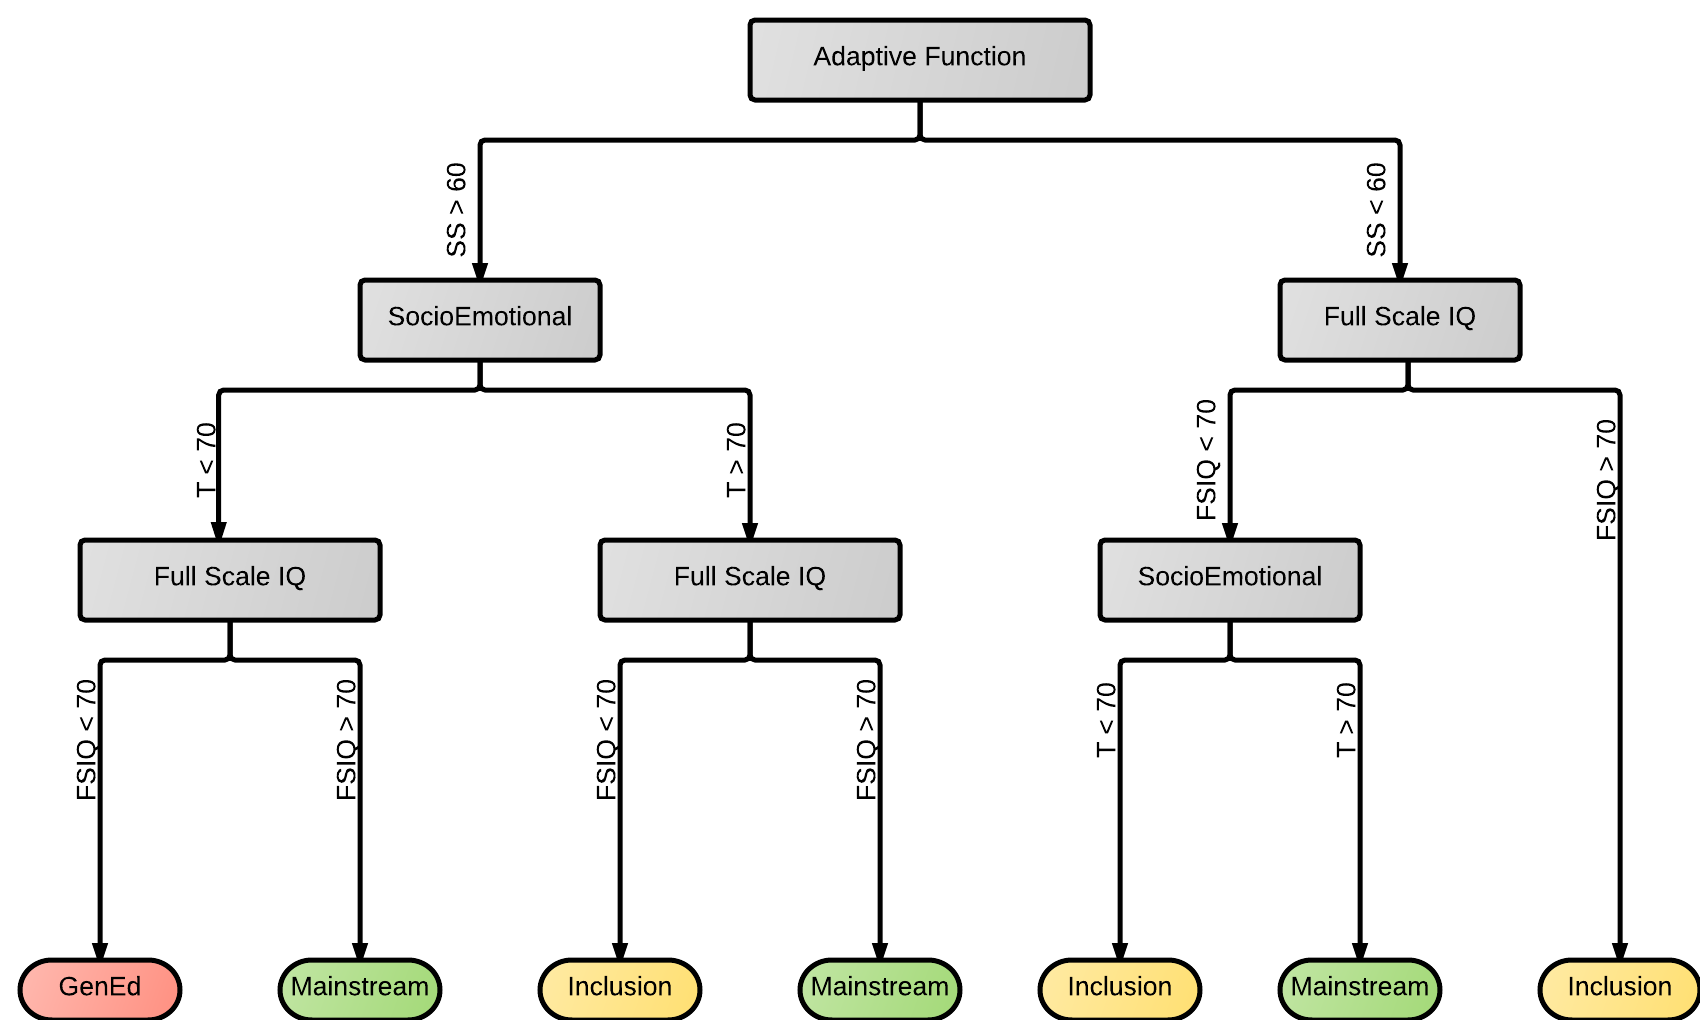
\includegraphics[width=\textwidth]{RegressionTree_NOAcademics.png}
	\caption[Mainstreaming Decision Tree]{\textit{           }}
	\label{fig1}
\end{figure*}
%
%%%%%%%%%%%%%%%%%%%%%%%%%%%%%%%%%%%%%%%%%%%%
%
% End Figure 1
%
%%%%%%%%%%%%%%%%%%%%%%%%%%%%%%%%%%%%%%%%%%%%
%
When academic information is included as means across the WJ-IIINU and CBM, CBM (indicating classroom performance) is the primary determining factor for success, followed by WJIII-NU and socioemotional function. FSIQ appears to only become involved when very low WJ-IIINU scores are present and there are some socioemotional difficulties.

%
%%%%%%%%%%%%%%%%%%%%%%%%%%%%%%%%%%%%%%%%%%%%
%
% Begin Figure 2
%
%%%%%%%%%%%%%%%%%%%%%%%%%%%%%%%%%%%%%%%%%%%%
%
\begin{figure*}[htp!]
	\centering
	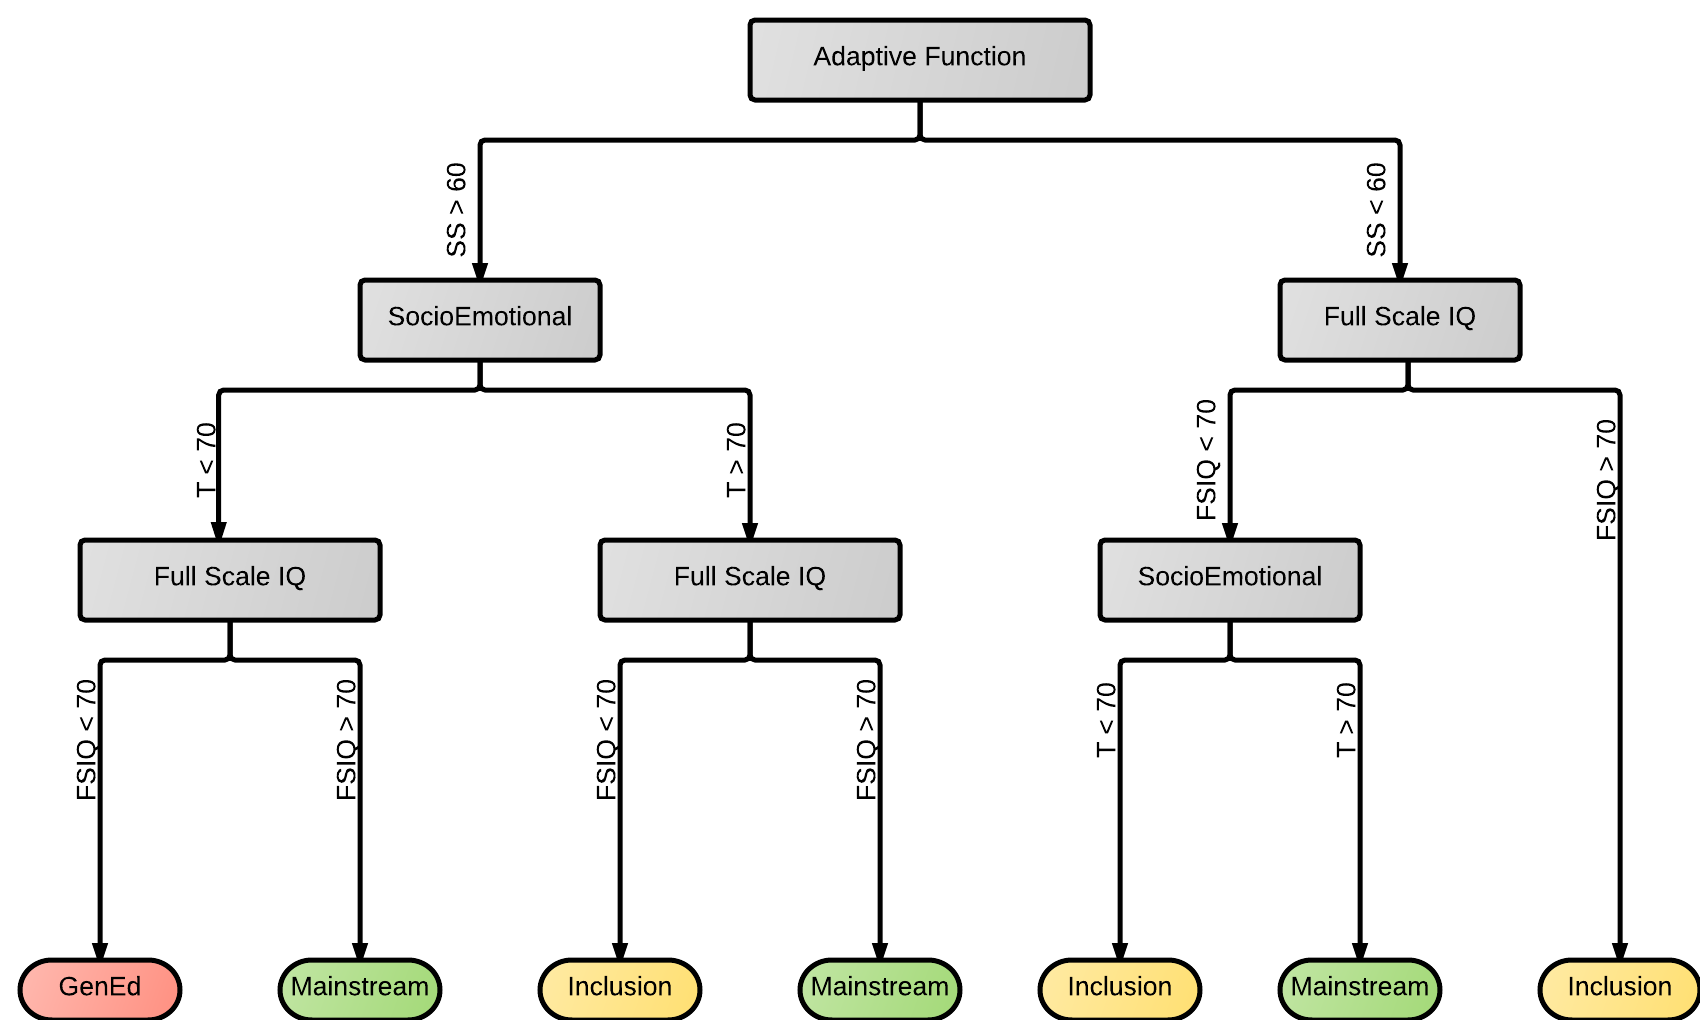
\includegraphics[width=\textwidth]{RegressionTree_NOAcademics.png}
	\caption[Mainstreaming Decision Tree]{\textit{          }}
	\label{fig2}
\end{figure*}
%
%%%%%%%%%%%%%%%%%%%%%%%%%%%%%%%%%%%%%%%%%%%%
%
% End Figure 2
%
%%%%%%%%%%%%%%%%%%%%%%%%%%%%%%%%%%%%%%%%%%%%
%
When academic information is included and all academic measures provided separately, a much more complicated picture appears. It appears that CBM math measures are most reliable for the initial split, followed by SocioEmotional data. Reading comprehension appears to be the most reliable indicator separating final general education placement relative to other factors. In separating inclusion from mainstreaming endpoints, it appears Basic Reading Skills are paramount. These data suggest that mathematics knowledge is critical, and after that Reading Comprehension. In the presence of poor CBM math scores, them math Reasoning becomes critical and  


\subsubsection{Hierarchal Cluster Analyses and Heatmaps}

The data presented in the heatmap in Figure ~\ref{fig3} that there was a 90\%+ correct classification of students designated for mainstreaming or inclusion. Interestingly, one can also see the Cognitive factors were separated from the academic factors, and CBM measurements were included as cognitive, rather than academic factors. 

These data all support the use of the Mainstreaming Decision Tree by reaching similar conclusions as to student allocation or classification as the Mainstreaming Decision Tree using a converging method, 
%
%%%%%%%%%%%%%%%%%%%%%%%%%%%%%%%%%%%%%%%%%%%%
%
% Begin Figure 3
%
%%%%%%%%%%%%%%%%%%%%%%%%%%%%%%%%%%%%%%%%%%%%
%
\begin{figure*}[htp!]
	\centering
	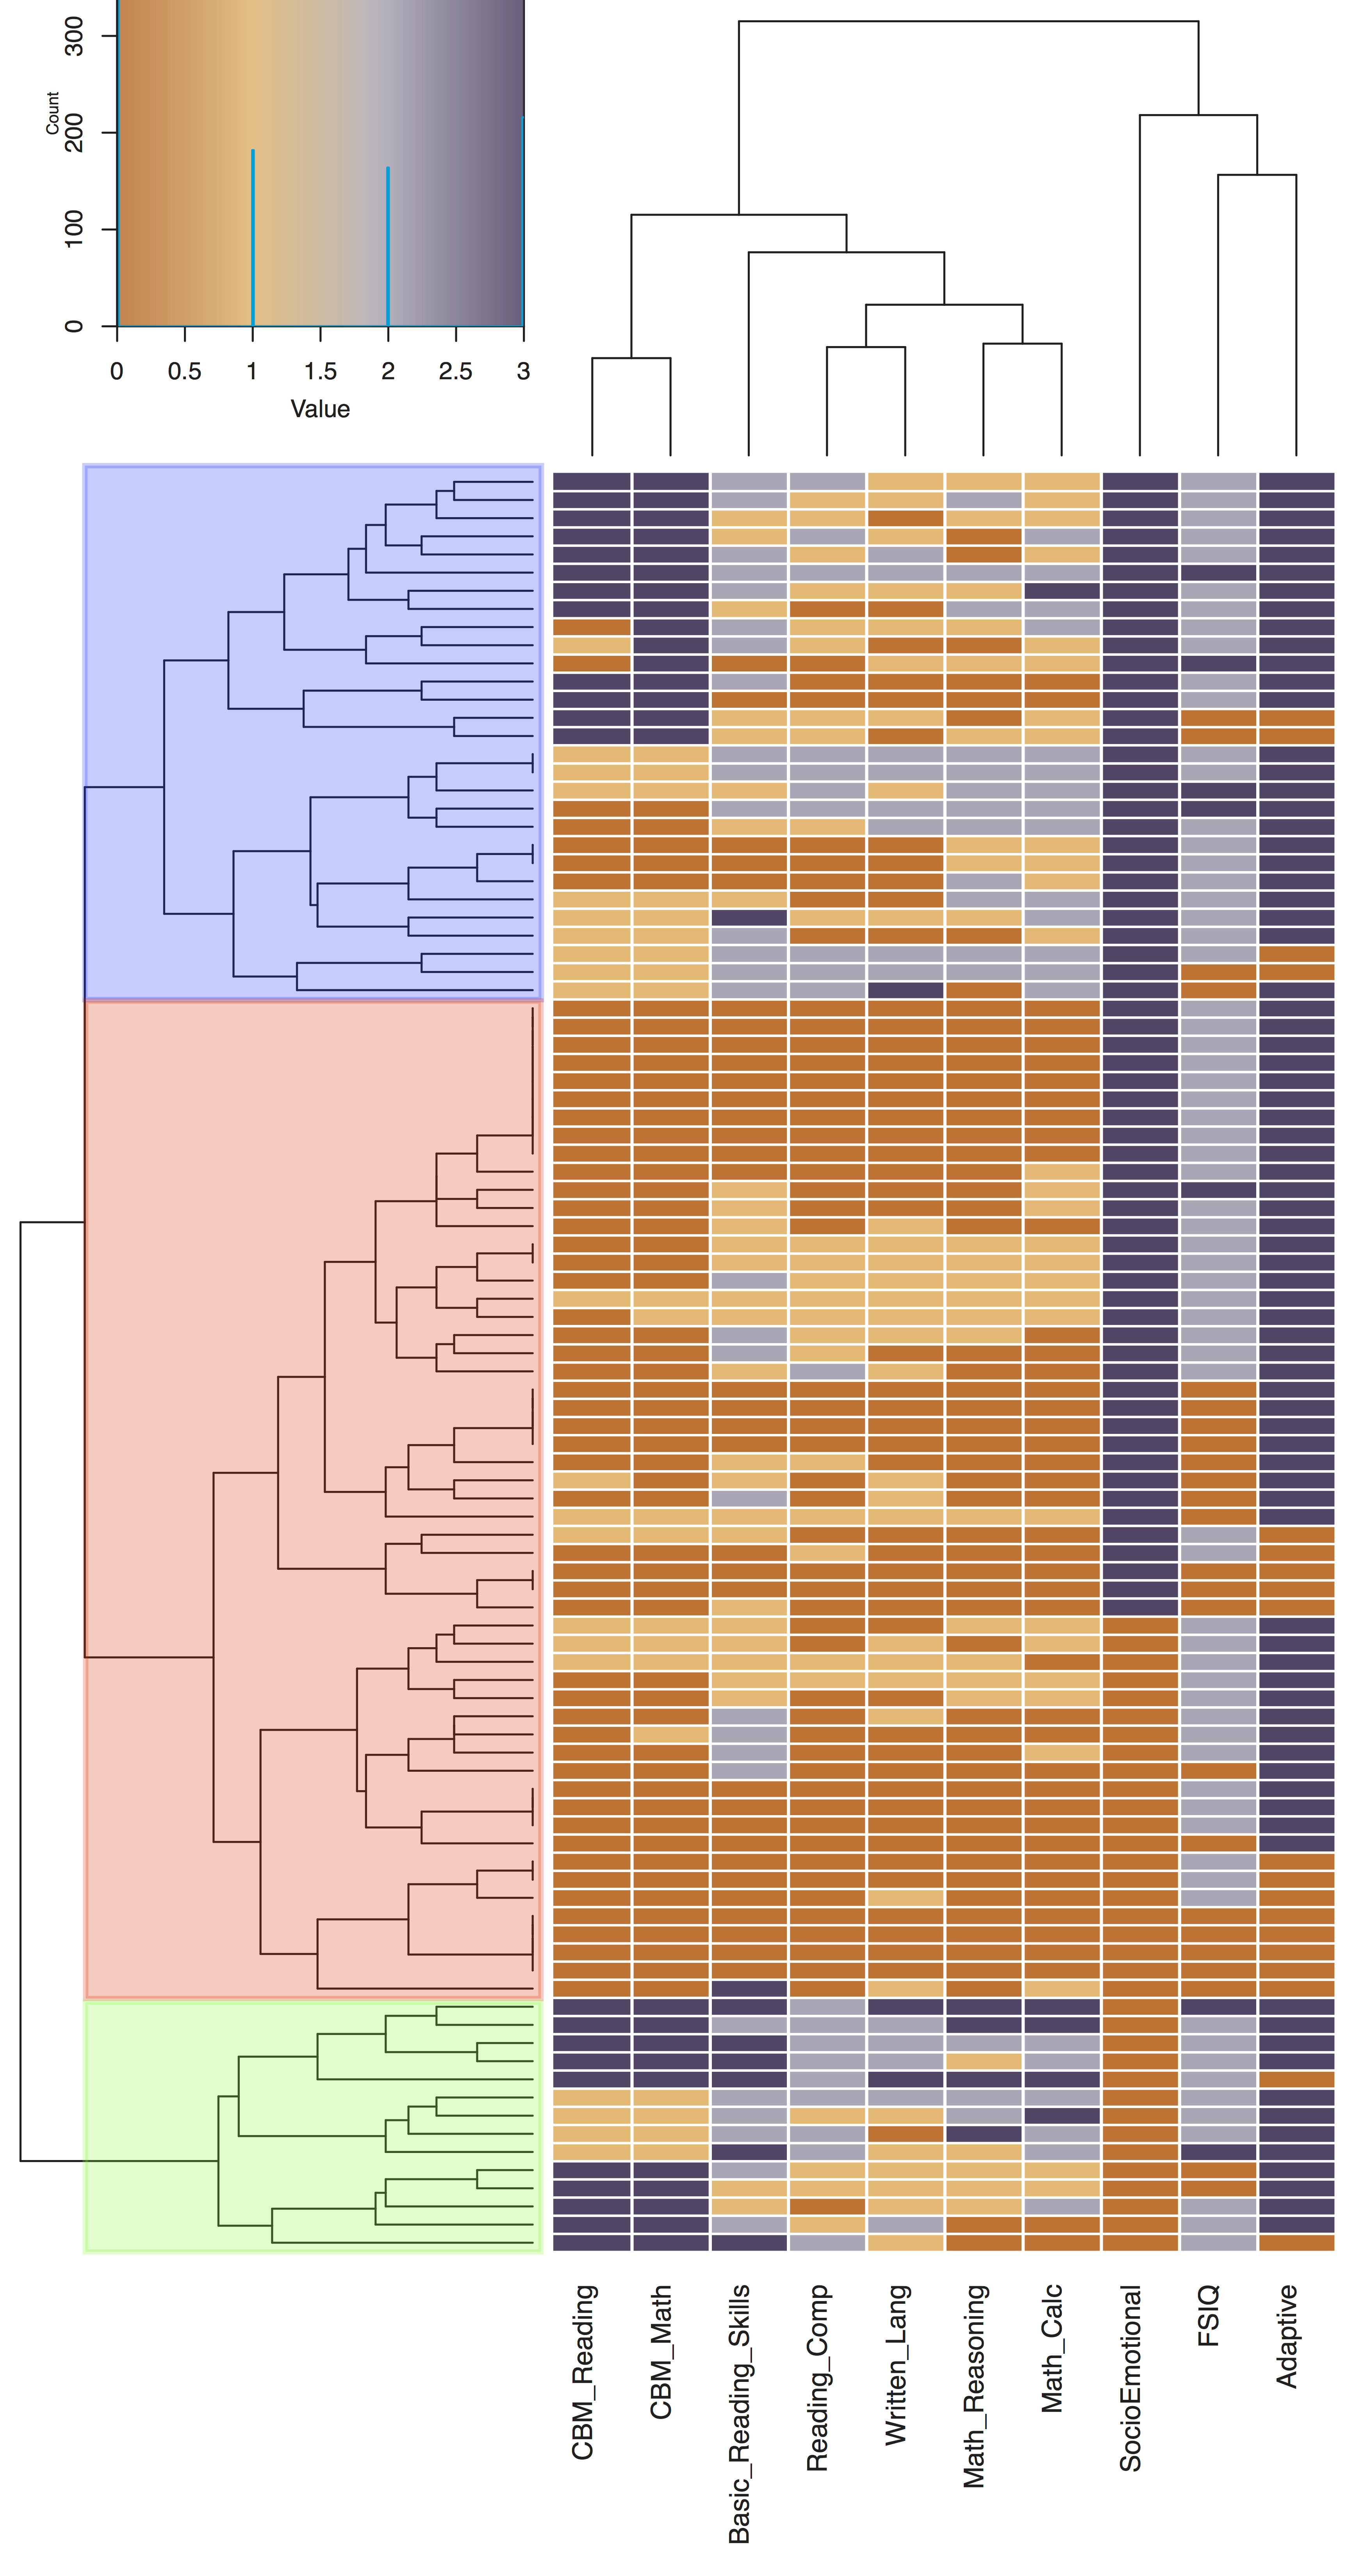
\includegraphics[width=\textwidth,height=\textheight]{Heatmap_Overall.png}
	\caption[Overall Predictive Results of Decision Algorithm]{\textit{           }}
	\label{fig3}
\end{figure*}
%
%%%%%%%%%%%%%%%%%%%%%%%%%%%%%%%%%%%%%%%%%%%%
%
% End Figure 3
%
%%%%%%%%%%%%%%%%%%%%%%%%%%%%%%%%%%%%%%%%%%%%
%

\subsubsection{Machine Learning Algorithm and Classification}

Note in Table~\ref{tab4} that the classifier mis-classified 1 General Education student as Mainstreaming and 0 as inclusion. 3 inclusion students were mis-classified as needing mainstreaming. 3 Mainstreaming students were misclassified as General Education and 2 were misclassified as requiring inclusion. These data are important because it means the algorithm is optimistic, erring on the side of moving the student to a less restrictive environment rather than favoring more restrictive environments. Also, these data by and large support the classroom decisions undertaken this past year, which was to favor moving students into less restrictive environments when they were approaching "ready", rather than waiting. 
%
%%%%%%%%%%%%%%%%%%%%%%%%%%%%%%%%%%%%%%%%%%%%
%
% Begin Table 3
%
%%%%%%%%%%%%%%%%%%%%%%%%%%%%%%%%%%%%%%%%%%%%
%
\begin{table}[tbp!]
	\centering
	\caption{Continuous to Categorical Value Mapping}
	\label{tab3}
	\begin{tabular}{ccccc}
		\hline \\
		Manual Placement $ \Rightarrow $ & General Education & Inclusion & Mainstreaming & \% Correct Classification\\
		\hline \\
		 SVM Prediction $ \Downarrow $ & & \\ \\
		General Education & 12 & 0 & 1 & 93\% \\
		Inclusion & 0 & 20 & 3 & 87\% \\
		Mainstream & 3 & 2 & 20 & 80\% \\
		\hline
	\end{tabular}
\end{table}
%
%%%%%%%%%%%%%%%%%%%%%%%%%%%%%%%%%%%%%%%%%%%%
%
% End Table 3
%
%%%%%%%%%%%%%%%%%%%%%%%%%%%%%%%%%%%%%%%%%%%%
%
%
%%%%%%%%%%%%%%%%%%%%%%%%%%%%%%%%%%%%%%%%%%%%
%
% Begin Table 4
%
%%%%%%%%%%%%%%%%%%%%%%%%%%%%%%%%%%%%%%%%%%%%
%
\begin{table}[tbp!]
	\centering
	\caption{Support Vector Machine Accuracies}
	\label{tab4}
	\begin{tabular}{p{5cm}p{8cm}p{5cm}}
		\hline \\
		X-Fold CV & Single Run Accuracies (\%) & Mean Accuracy (\%)\\
		\hline \\
		30 fold CV & 100, 66.67, 100, 100, 100 \newline 66.67, 100, 100, 66.67, 100 \newline 100, 100, 100, 66.67, 100 \newline 66.67, 100, 100, 75, 66.67 \newline 66.67, 100, 100, 100, 66.67 \newline 33.33, 75, 33.33, 100, 100 & 85.71\\ \\
		20 fold CV   & 75, 60, 80, 100, 80 \newline 80, 80, 80, 100, 80 \newline 75, 100, 60, 60, 100 \newline 100, 100, 100, 100, 80& 84.69 \\ \\
		10 fold CV   & 88.89, 90, 100, 80, 70 \newline 66.67, 80, 90, 80, 90& 83.67 \\ \\
		5 fold CV  & 78.95, 85, 89.47, 90, 85 & 85.71 \\ \\ 
		3 fold CV   & 81.25, 87.88, 81.82 & 83.67 \\ \\
		\multicolumn{2}{r}{Overall Mean} & 84.69 $ \pm $ 1.02\% SD \\ 
		\hline
	\end{tabular}
\end{table}
%
%%%%%%%%%%%%%%%%%%%%%%%%%%%%%%%%%%%%%%%%%%%%
%
% End Table 4
%
%%%%%%%%%%%%%%%%%%%%%%%%%%%%%%%%%%%%%%%%%%%%
%

\section{Discussion}
%
%
%
%
%


%\clearpage
\printbibliography
\clearpage
%\appendix
%\appendixpage
%\section{Mainstreaming Decision Tree - Academics}
%\section{Mainstreaming Decision Tree - Behavior}
%\section{Mainstreaming Plan Form}
%\section{Classroom Ecological Inventory (K-6)}
%\section{Behavioral First Aid Kit}
%\label{Appendix1}
%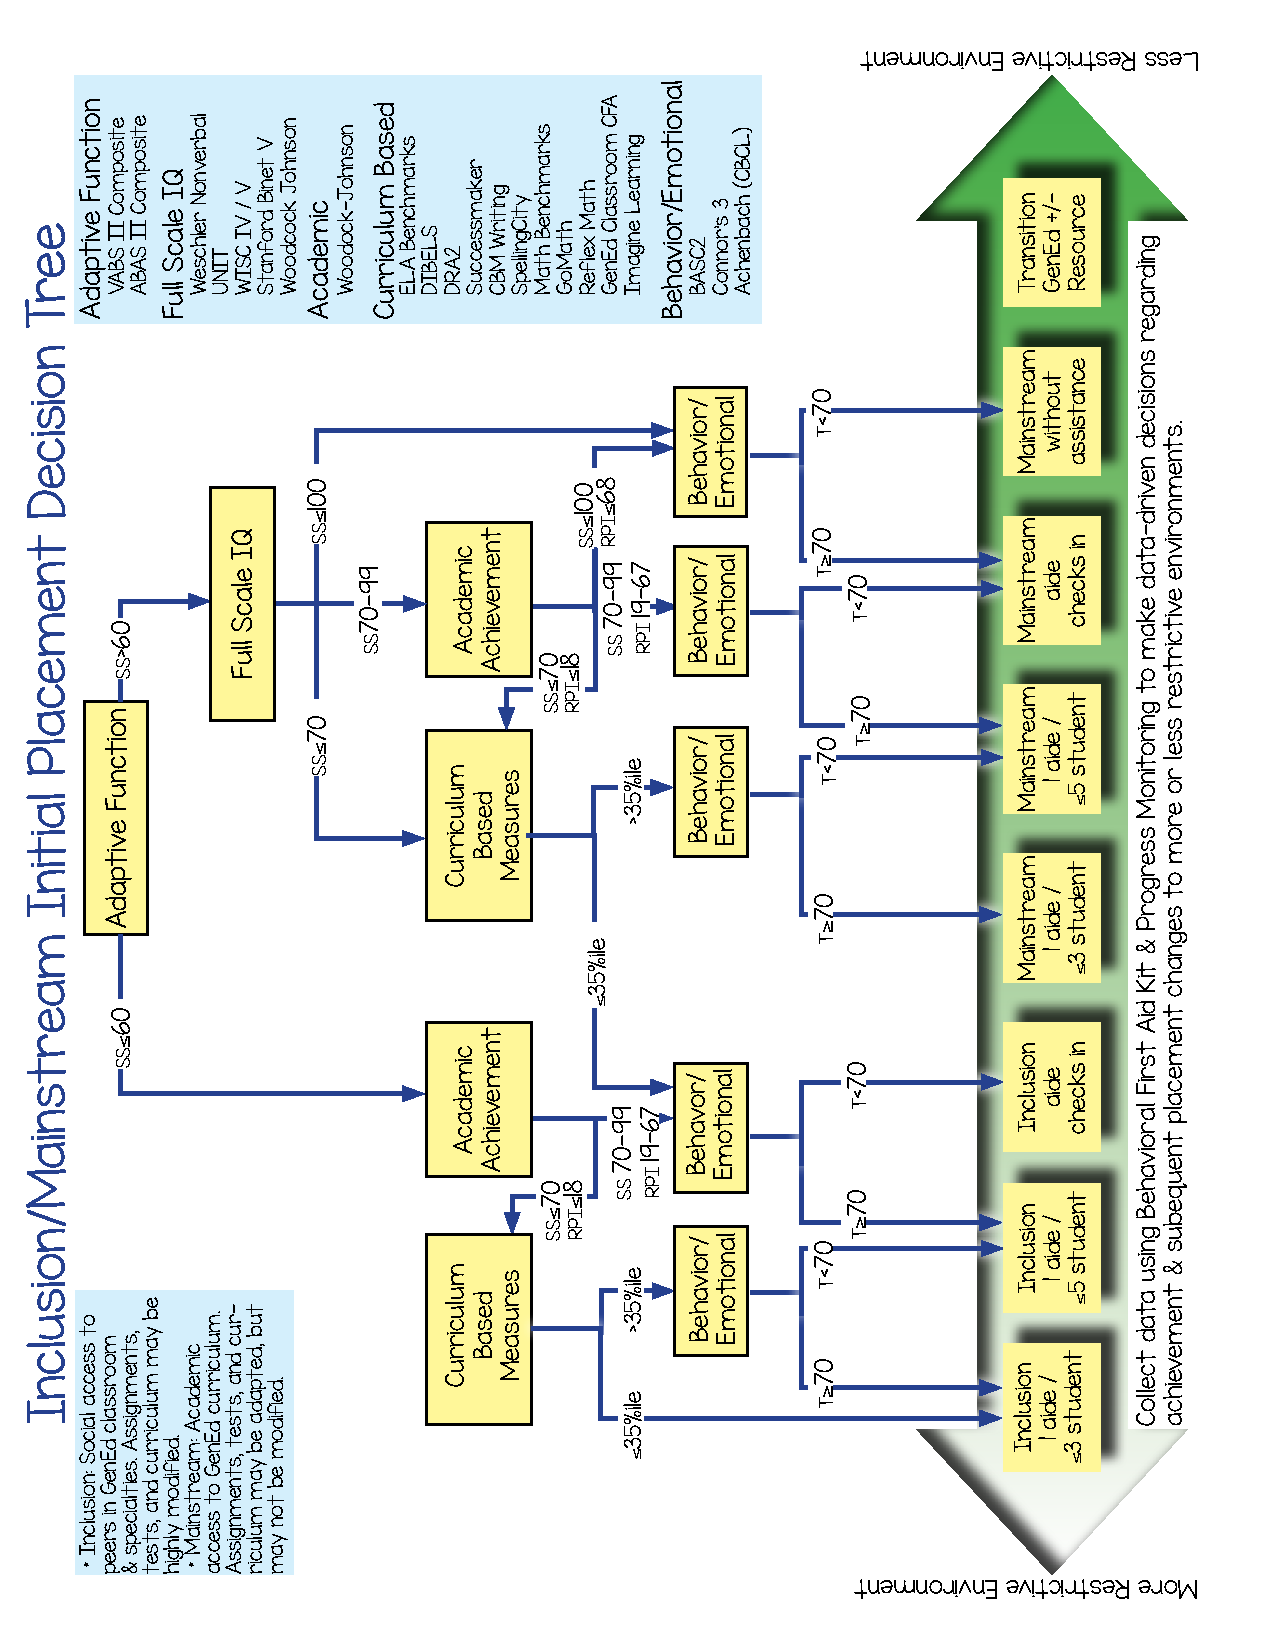
\includepdf[landscape=TRUE, pages={1}]{DecisionTree.pdf}
%\label{Appendix2}
%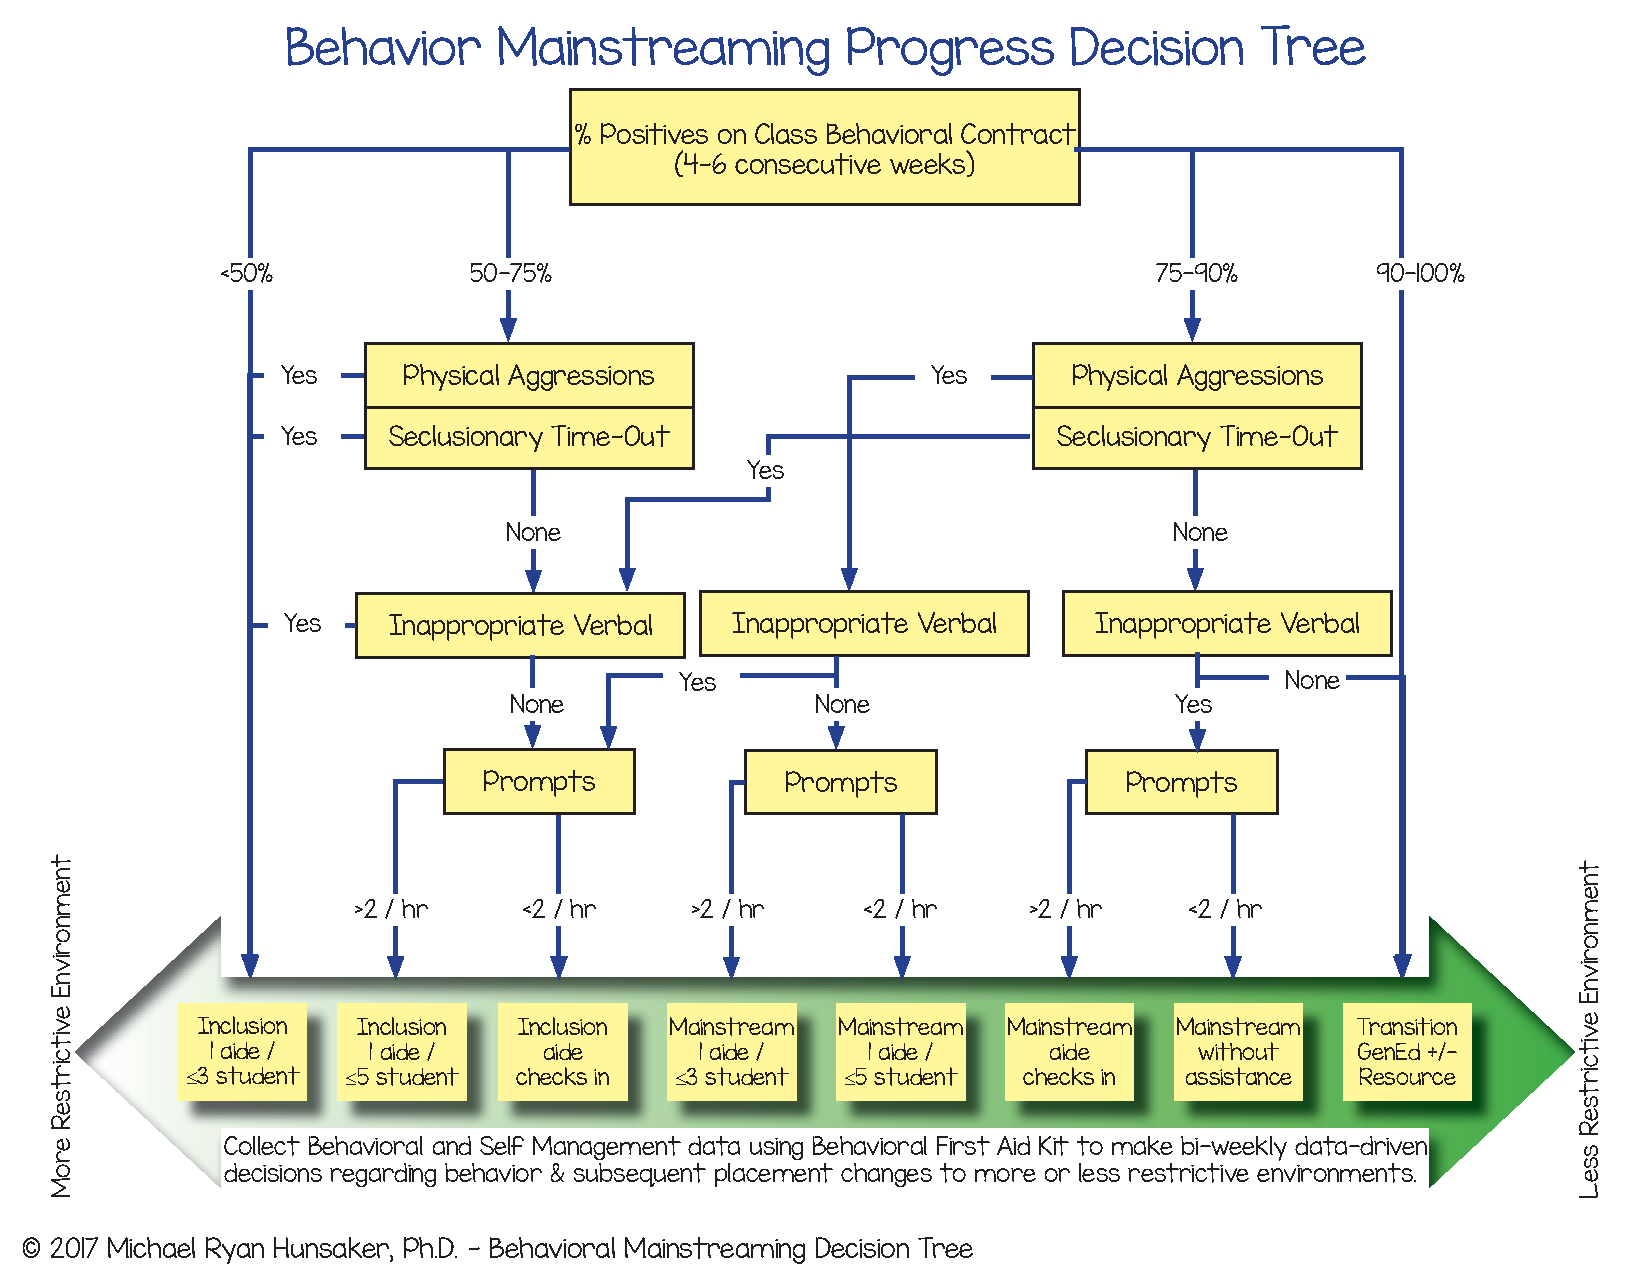
\includepdf[landscape=TRUE, pages={1}]{BehaviorPipeline.pdf}
%\label{Appendix3}
%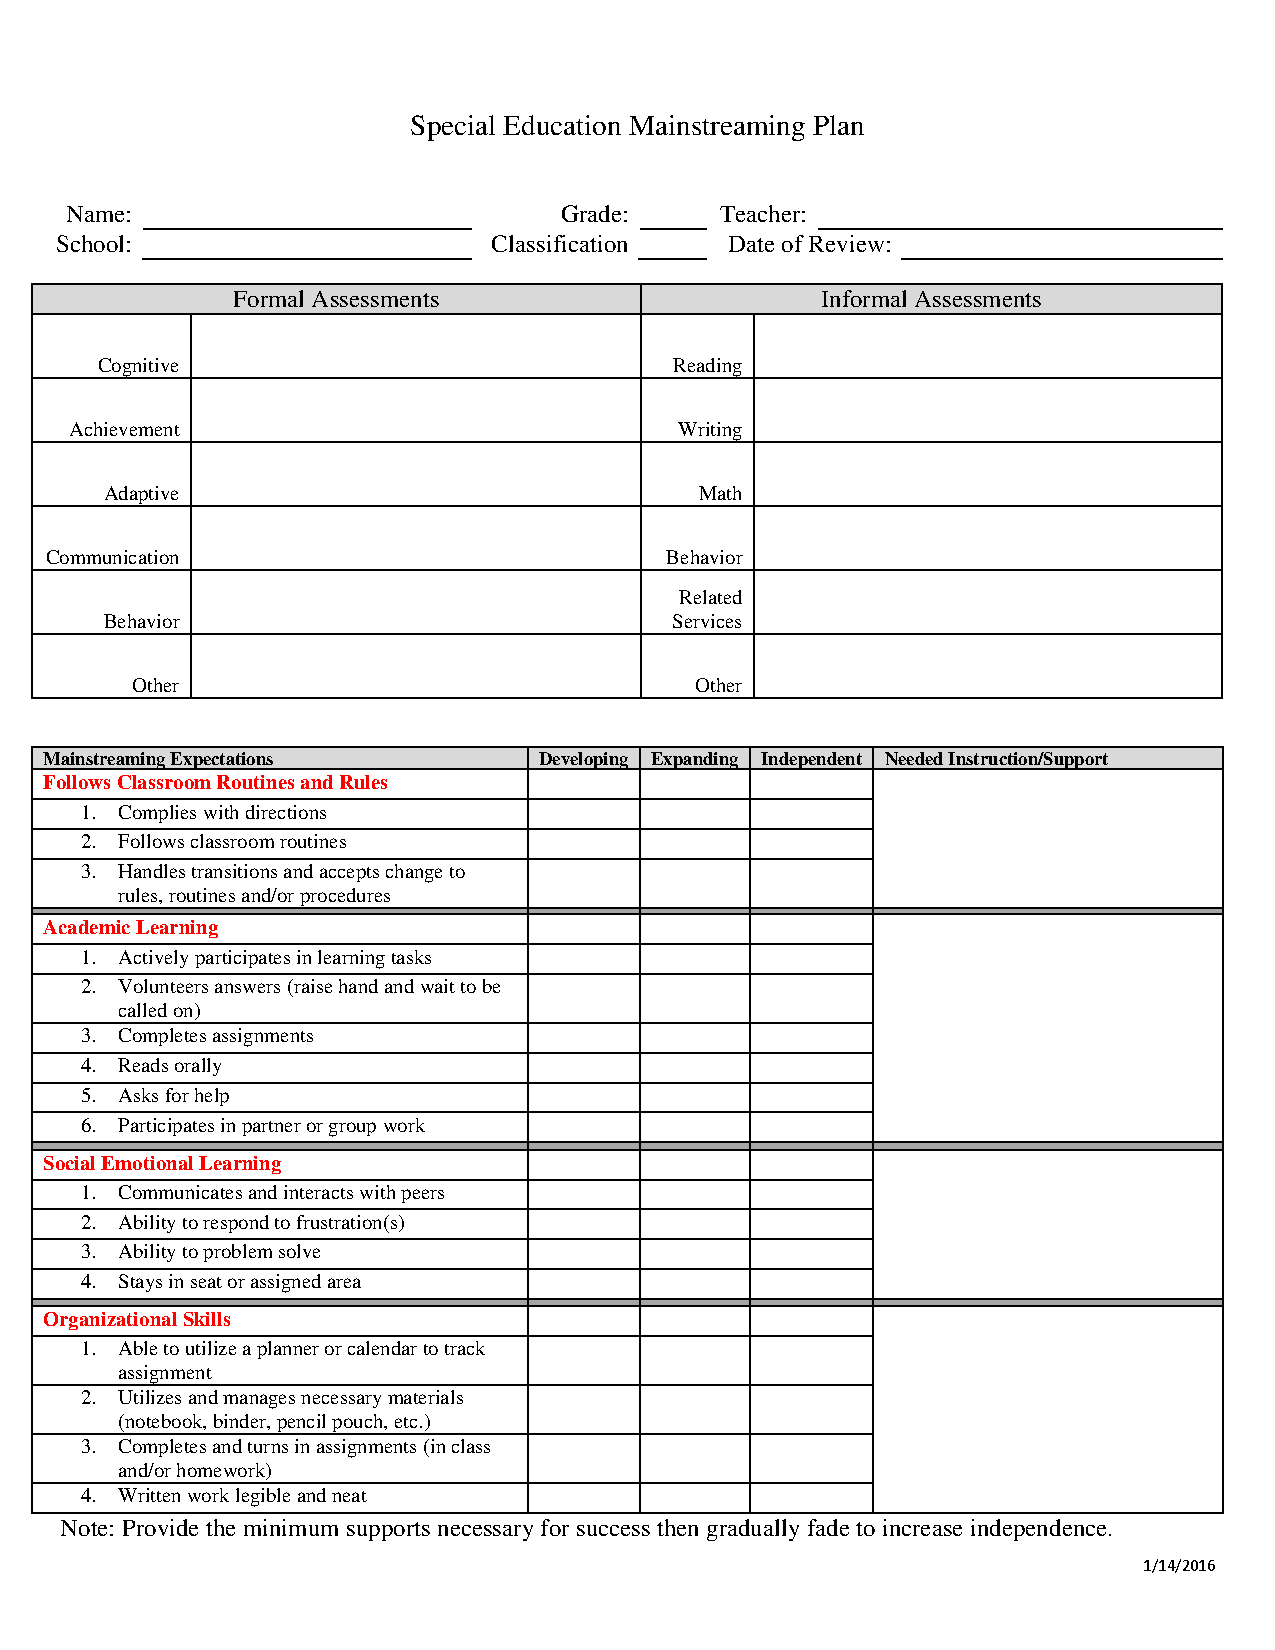
\includepdf[pages={1,2}]{MainstreamingPlan.pdf}
%\clearpage \mbox{} \clearpage
%\label{Appendix4}
%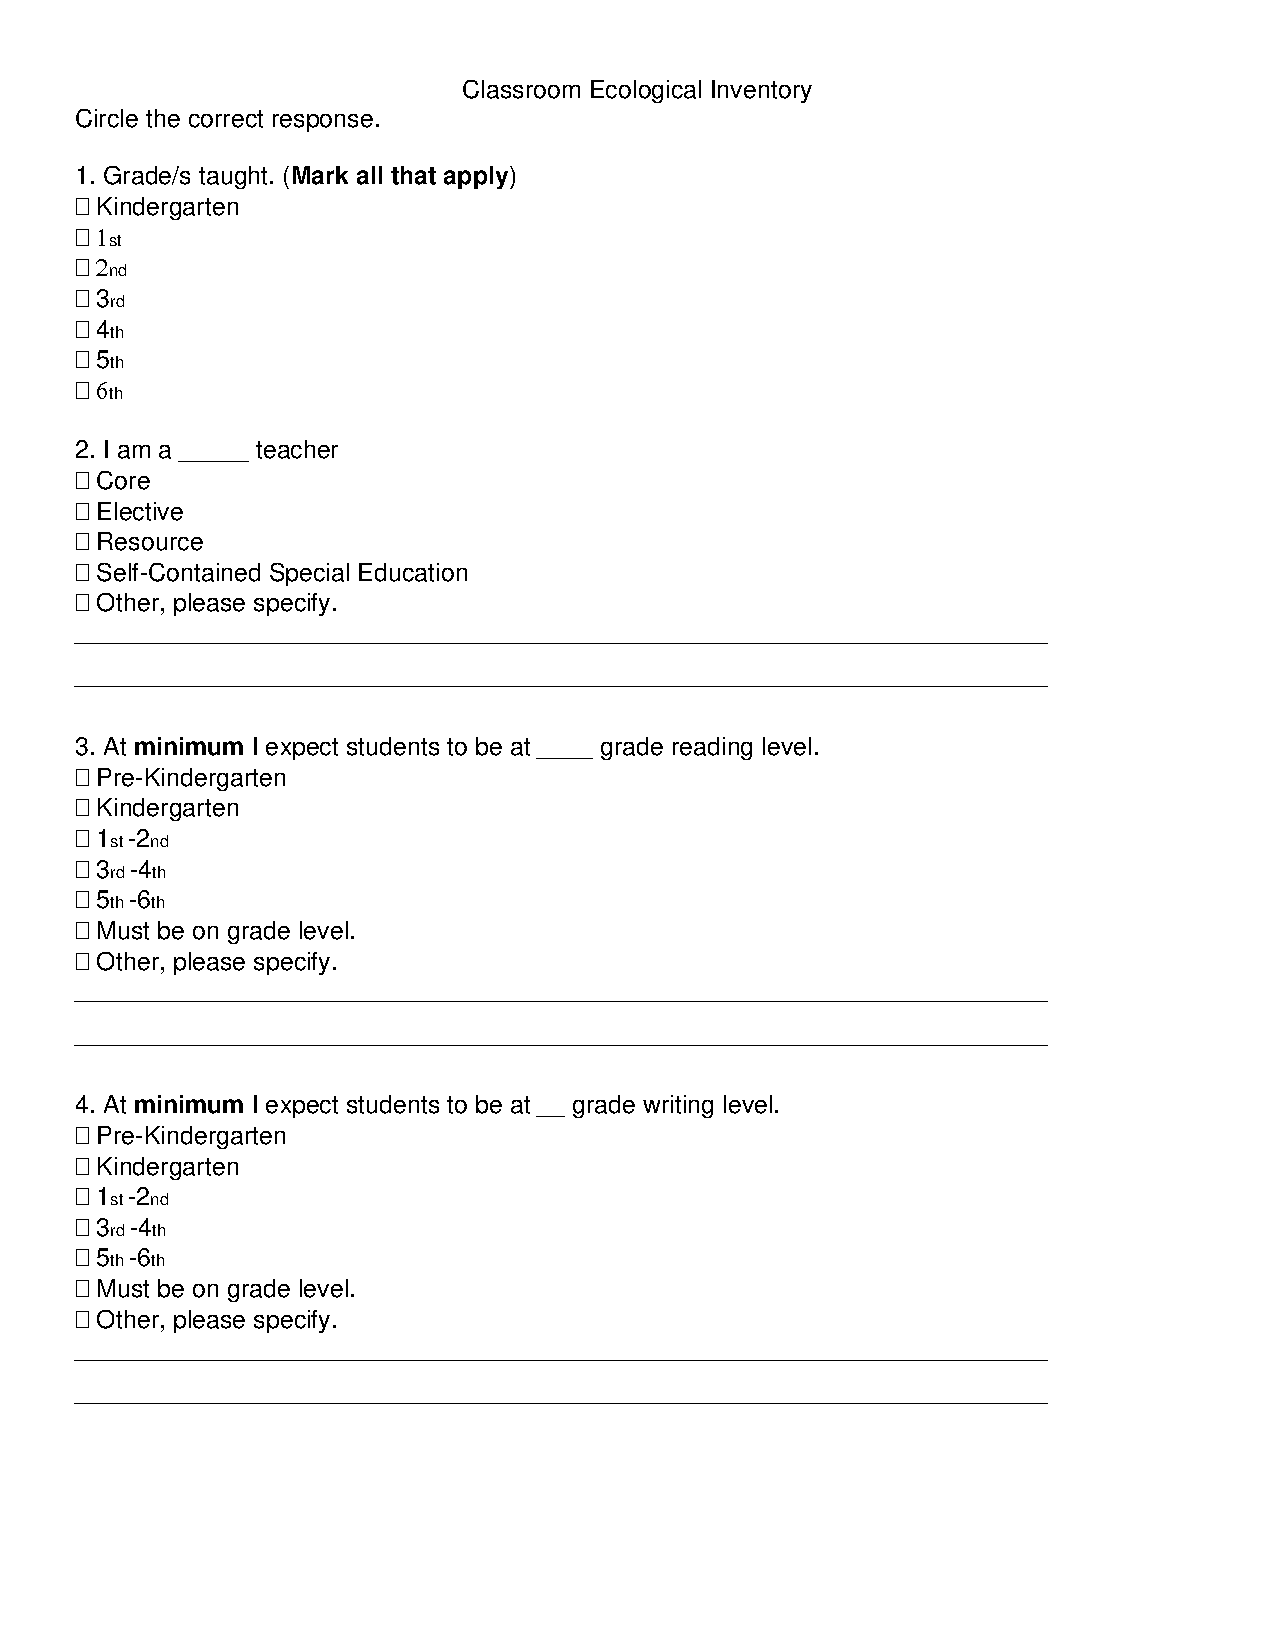
\includepdf[pages={1,2,3,4,5}]{ClassroomEcologicalInventory.pdf}
%\clearpage \mbox{} \clearpage
%\label{Appendix5}
%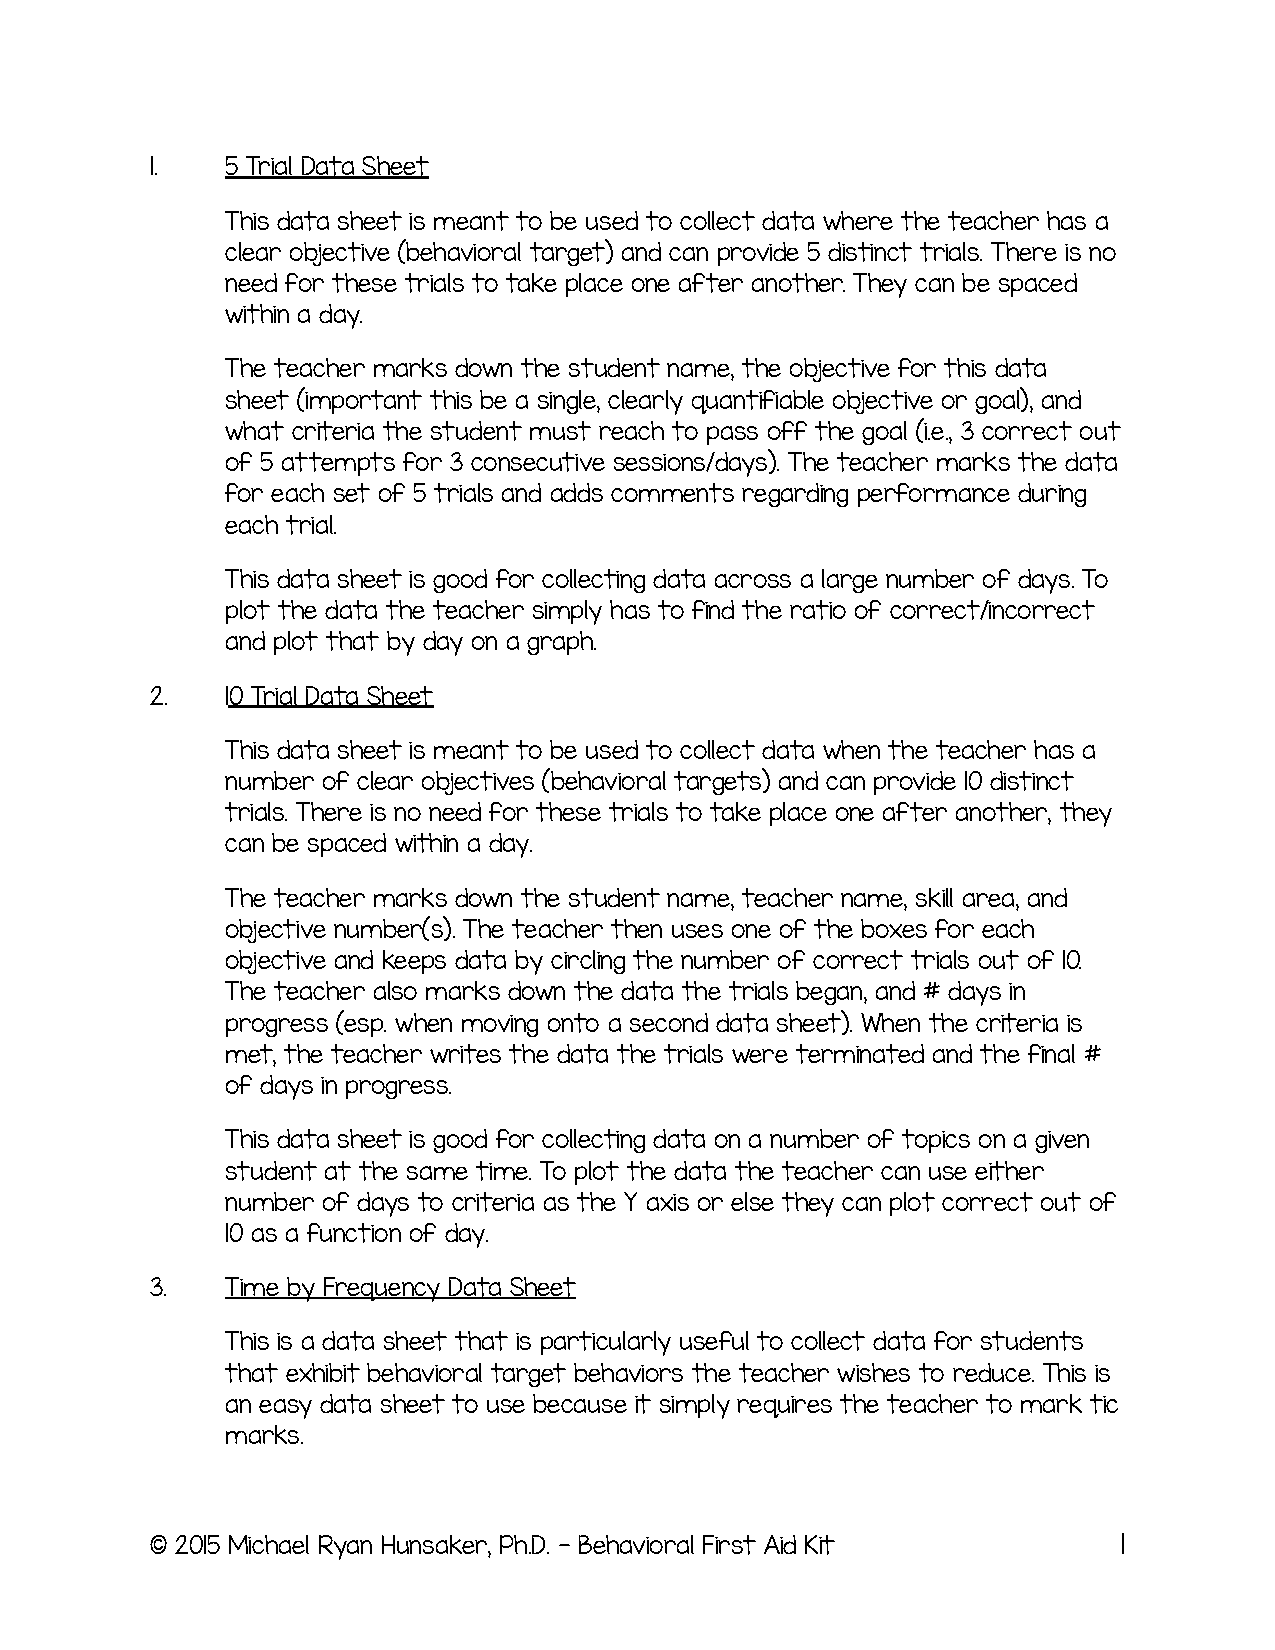
\includepdf[pages={1-56}]{BehavioralFirstAidKit.pdf}
%%%%%%%%%%%%%%%% End Body %%%%%%%%%%%%%%%%%%%%%%%
%
%%%%%%%%%%%% Begin Back Matter %%%%%%%%%%%%%%%%%%%
%\addcontentsline{toc}{part}{Notes and Bioliography}
\end{document}